% -*- TeX -*- -*- US -*-
\documentclass{article} % For LaTeX2e
\usepackage{nips13submit_e,times}
\input{sl_preamble.tex}
\input{sl_graphics_preamble.tex}
\graphicspath{{"Figs/"}}
% >> Only for drafts! <<
\usepackage[notref,notcite]{showkeys}
% ----------------------------------------------------------------
%\numberwithin{equation}{section}
%\renewcommand{\baselinestretch}{1.5}
% ----------------------------------------------------------------
% New commands etc.
\input{sl_definitions.tex}
\input{sl_symbols.tex}
%
%additional symbols:
%
\DeclareMathOperator{\SNR}{SNR}
\DeclareMathOperator{\snr}{SNR}
\newcommand{\wv}{\vec{w}}
\newcommand{\wvi}{\vec{w}_\text{ideal}}
%matrices
\newcommand{\inv}{^{-1}}
\newcommand{\dg}{^\mathrm{dg}}
\newcommand{\trans}{^\mathrm{T}}
\newcommand{\I}{\mathbf{I}}
%vec of ones
\newcommand{\onev}{\mathbf{e}}
%mat of ones
\newcommand{\onem}{\mathbf{E}}
%Markov matrix
\newcommand{\MM}{\mathbf{Q}}
%prob distributions
\newcommand{\pr}{\mathbf{p}}
\newcommand{\eq}{\pr^\infty}
%first passage times
\newcommand{\fpt}{\mathbf{T}}
%off-diag first passage times
\newcommand{\fptb}{\overline{\fpt}}
%fundamental matrix
\newcommand{\fund}{\mathbf{Z}}
%other symbols for matrices
\newcommand{\Pb}{\mathbf{P}}
\newcommand{\D}{\mathbf{D}}
\newcommand{\pib}{\boldsymbol{\pi}}
\newcommand{\Lb}{\boldsymbol{\Lambda}}
\newcommand{\w}{\mathbf{w}}
\newcommand{\W}{\mathbf{W}}
\newcommand{\M}{\mathbf{M}}
\newcommand{\enc}{\mathbf{q}}
\newcommand{\frg}{\W^{\mathrm{F}}}
\newcommand{\F}{\boldsymbol{\Phi}}
%superscripts
\newcommand{\pot}{^{\text{pot}}}
\newcommand{\dep}{^{\text{dep}}}
\newcommand{\potdep}{^{\text{pot/dep}}}
%sets
\newcommand{\CS}{\mathcal{S}}
\newcommand{\CA}{\mathcal{A}}
\newcommand{\CB}{\mathcal{B}}
\newcommand{\comp}{^\mathrm{c}}
%eigenmodes
\newcommand{\uv}{\mathbf{u}}
\newcommand{\vv}{\mathbf{v}}
\newcommand{\CI}{\mathcal{I}}

%
%%%%%%%%%%%%%%%%%%%%%%%%%%%%%%%%%%%%%%%%%%%%%%%%%%%%%%%%%%%%%%%%%%%%%%%%%%
% Title info:
\title{A memory frontier for complex synapses}
%
% Author List:
%
\author{Subhaneil Lahiri and Surya Ganguli\\
Applied Physics Department, Stanford University, Stanford CA\\
\emaillink{sulahiri@stanford.edu}, \emaillink{sulahiri@stanford.edu}
%
}

%\nipsfinalcopy % Uncomment for camera-ready version

\begin{document}

\maketitle


%%%%%%%%%%%%%%%%%%%%%%%%%%%%%%%%%%%%%%%%%%%%%%%%%%%%%%%%%%%%%%%%%%%%%%%%%%


\begin{abstract}
  Blah blah blah.
\end{abstract}


%%%%%%%%%%%%%%%%%%%%%%%%%%%%%%%%%%%%%%%%%%%%%%%%%%%%%%%%%%%%%%%%%%%%%%%%%%

\section{Introduction}\label{sec:intro}

In the field of theoretical neuroscience there are several classic results regarding the storage capacity of synaptic memory, \eg the Hopfield model's capacity is proportional to the number of neurons, or the Perceptron's capacity is proportional to the number of synapses.
However, these rely on one unrealistic feature of these models: the synaptic weights are allowed to take a large number of different values.

Measurements of real synapses have shown that the synaptic efficacy can only take a small number of discrete values, possibly as few as two \cite{Bliss1993LTP,Petersen1998allornone,O'Connor2005switch} (see \cite{Enoki2009graded} for dissenting results).
Restricting synaptic weights to a small set of values has a catastrophic effect on the storage capacity of these theoretical models, growing only logarithmically with the size of the system if all else is held fixed \cite{amit1992constraints,amit1994learning}.
Due to newer memories overwriting older ones, there is a trade-off between learning and remembering: if synapses are too plastic older memories will be wiped out too easily, if they are too rigid it becomes difficult to learn new memories in the first place.

This can be improved when we take into account the fact that there is a complex dynamical system underlying synaptic plasticity (\eg see \cite{Bliss1993LTP,Bredt2003AMPA,Coba2009phosphorylation}).
Allowing the synapse to have hidden functional states, with potentiation and depression causing transitions between these states, can dramatically improve their performance.

Much of the previous work on these types of synaptic models has focussed on specific models, to understand their ability to store memories \cite{Fusi2005cascade,Fusi2007multistate,Leibold2008serial}.
Two examples of these models are shown in \autoref{fig:models}.
we see that they have different memory properties.
The serial model has performs very well at one particular timescale, but it performs poorly at other times.
The cascade model does not perform quite as well at that time, but it maintains it performance over a wider range of timescales.


\begin{figure}[tbp]
 \begin{center}
 \begin{myenuma}
  \item\aligntop{\includegraphics[width=0.25\linewidth]{cascade.svg}}\label{fig:cascade}
  \item\aligntop{\includegraphics[width=0.25\linewidth]{multistate.svg}}\label{fig:multistate}
  \item\aligntop{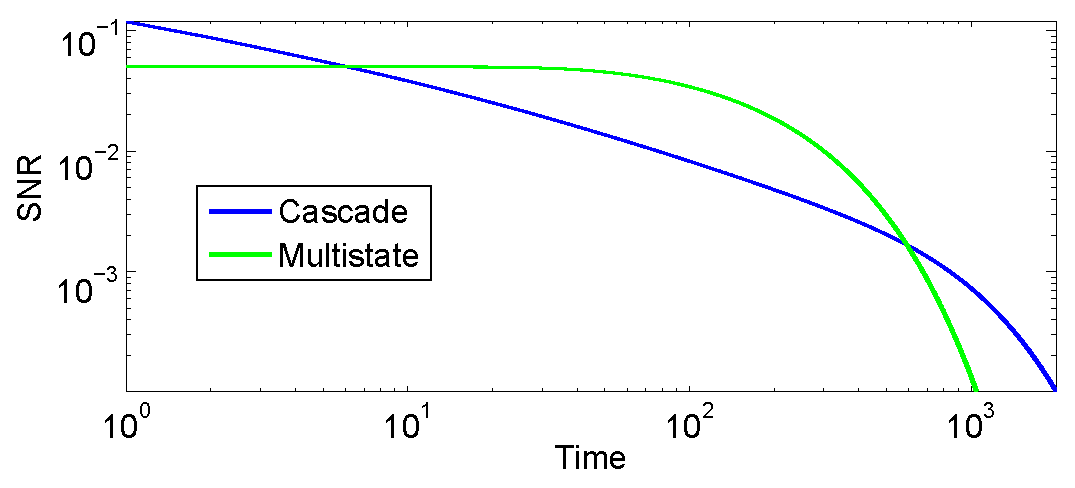
\includegraphics[width=0.35\linewidth]{cascms.eps}}\label{fig:cascms}
 \end{myenuma}
 \end{center}
  \caption{Models of complex synapse.
  (\ref{fig:cascade}) The cascade model of \cite{Fusi2005cascade}, showing transitions between states of high/low synaptic weight (red/blue circles) due to potentiation/depression (solid red/dashed blue arrows).
  (\ref{fig:multistate}) The serial model of \cite{Leibold2008serial}.
  (\ref{fig:cascms}) The memory curves of these two models, showing the decay of the signal-to-noise ratio (to be defined in \autoref{sec:setup}) as subsequent memories are stored.
  }\label{fig:models}
\end{figure}



We are going to take a different approach.
We are going to consider the \emph{entire} space of these models to find upper bounds on the capability of \emph{any} of them.
As the performance of a synaptic model is quantified by a memory curve (describing the decay of a memory trace as more and more subsequent memories are stored) rather than a single number, there is no good notion of optimality.
What type of memory curve is best will depend on what the synapses are required to do and over what timescales.

We begin in \autoref{sec:setup} by describing the class of models that we will consider and define the memory curve that we use to quantify their performance.
In \autoref{sec:bounds} we will prove upper bounds on two quantities, the initial value of the memory curve and the area under it, as well as finding the models that saturate them.
We will use these bounds in \autoref{sec:env} to find an envelope curve -- one that cannot be crossed by the memory curve of any model at any time.




\section{Synaptic models and their memory curves}\label{sec:setup}

In this section, we will describe the class of models of synaptic plasticity that we are studying and how we quantify their performance as memory storage devices.
In the subsequent sections, we will find upper bounds on this performance.

We use a well established formalism for the study of learning and memory with complex synapses (see \cite{Fusi2005cascade,Fusi2007multistate,Barrett2008discrete}).
In this approach, potentiating and depressing plasticity events occur at random times, with all information about the neural activity and learning rules responsible for them absorbed into their rates.
We assume that there are no spatial or temporal correlations in the pattern of potentiating and depressing events, and these events cause Markovian transitions between the internal states of the synapses.
As a result of these assumptions, the states of different synapses will be independent, and the system can be fully described by the probability distribution across these states, which we will indicate with the row-vector $\pr(t)$.

We also employ an ``ideal observer'' approach to the memory readout, where the synaptic weights are read directly.
This provides an upper bound to the quality of any readout using neural activity.
These synaptic weights will be restricted to two values, which we can shift and scale to $\pm1$.

For any single memory, there will be an ideal pattern of synaptic weights, the $N$-element vector $\wvi$, that is $+1$ at all synapses that were potentiated and $-1$ at all synapses that were depressed.
The actual pattern of synaptic weights at some later time, $t$, will be $\wv(t)$.
We can use the overlap between these, $\wvi\cdt\wv(t)$, as a measure of the quality of the memory.
As $t\to\infty$, the system will return to its steady state distribution which will be uncorrelated with the memory in question.
The probability distribution of the quantity $\wvi\cdt\wv(\infty)$ can be used as a ``null model'' for comparison.

The extent to which the memory has been stored is described by a signal-to-noise ratio (SNR):
%
\begin{equation}\label{eq:SNRdef}
  \snr(t) = \frac{\av{\wv_\text{ideal}\cdt\wv(t) - \wv_\text{ideal}\cdt\wv(\infty)}}
     {\sqrt{\var(\wv_\text{ideal}\cdt\wv(\infty))}}.
\end{equation}
%
The noise is essentially $\sqrt{N}$.
There is a correction when potentiation and depression are imbalanced, but this will not affect the upper bounds that we will discuss below and will be ignored in the subsequent formulae.

All of the preceding plasticity events will put the system in its steady-state distribution, $\eq$.
The memory we are tracking at $t=0$ will change this to $\eq\M\pot$ in those synapses that are potentiated and $\eq\M\dep$ in those synapses that are depressed, where $\M\potdep$ are $M\times M$ matrices of transition probabilities for the Markov processes describing potentiation and depression.
As the potentiating/depressing nature of the subsequent memories is independent of $\wvi$, we can average over all sequences, resulting in the evolution of the probability distribution:
%
\begin{equation}\label{eq:evol}
  \diff{\pr(t)}{t} = r\pr(t)\frg,
  \qquad \text{where} \quad
  \frg = f\pot\M\pot + f\dep\M\dep - \I.
\end{equation}
%
Here, $r$ is the rate of the Poisson process describing the timing of plasticity events,
$f\potdep$ is the fraction of events that are potentiating/depressing and $\I$ is the identity matrix.

This results in the following SNR
%
\begin{equation}\label{eq:SNRcalc}
  \snr(t) = \sqrt{N}\prn{2 f\pot f\dep} \eq \prn{\M\pot-\M\dep} \e^{rt\frg} \w,
\end{equation}
%
where the weight of the synapse when it is in its $i$'th state is given by the corresponding element of the column vector $\w$.
We will frequently refer to this function as the memory curve.

The parameters must satisfy the following constraints:
%
\begin{equation}\label{eq:constr}
\begin{aligned}
  \M\potdep_{ij} &\in [0,1], &\quad
  f\potdep &\in [0,1], &\quad
  \eq\frg &= 0, &\quad
  \w_i &= \pm 1, \\
  \sum_j \M\potdep_{ij} &= 1, &
  f\pot + f\dep &= 1, &
  \sum_i \eq_i &= 1.
\end{aligned}
\end{equation}
%
The upper bounds on $\M\potdep_{ij}$ and $f\potdep$ follow automatically from the other constraints.

The question is: what do these constraints imply for the memory curve above?
In practice, to make any statements about finite times, we need to got to the eigenmode description:
%
\begin{equation}\label{eq:eigendecomp}
  \frg = \sum_a -q_a \uv^a \vv^a,
  \quad
  \vv^a \uv^b = \delta_{ab},
  \quad
  \frg \uv^a = -q_a \uv^a,
  \quad
  \vv^a \frg = -q_a \vv^a.
\end{equation}
%
Where $q_a$ are the negative of the eigenvalues, $\uv^a$ are the right (column) eigenvectors and $\vv^a$ are the left (row) eigenvectors.
This allow us to write
%
\begin{equation}\label{eq:SNReigen}
\begin{aligned}
  \snr(t) &= \sqrt{N}\sum_a \CI_a \e^{-rt/\tau_a},
  &\quad \text{where}&\;&
  \CI_a &= \prn{2 f\pot f\dep} \eq (\M\pot-\M\dep) \uv^a  \vv^a \w,\\&
  & \text{and}&&
  \tau_a &= \frac{1}{q_a}.
\end{aligned}
\end{equation}
%
We can ask then ask the question: what are the constraints on these quantities implied by the constraints \eqref{eq:constr}?
We will find some of these constraints in the next section.





\section{Upper bounds}\label{sec:bounds}

In this section, we will find some upper bounds on certain properties of the memory curve discussed in the previous section, namely its initial value and the area under it.
We will use these bounds to determine an upper bound on the SNR at finite times in the next section.


\subsection{Initial SNR}\label{sec:initial}

Now we will discuss the SNR at $t=0$:
%
\begin{equation}\label{eq:init}
  \snr(0) = \sqrt{N}\prn{2 f\pot f\dep} \eq \prn{\M\pot-\M\dep} \w.
\end{equation}
%
We will find an upper bound on this quantity for \emph{all} possible models and also find the model that saturates this bound.
As maximizing initial SNR does not place any value on later parts of the memory curve, this will produce models with fast decay that may not be good for memory storage.
Nevertheless, the upper bound will be useful in \autoref{sec:env}.

A useful quantity is the equilibrium probability flux between two disjoint sets of states, $\CA$ and $\CB$:
%
\begin{equation}\label{eq:flux}
  \F_{\CA\CB} = \sum_{i\in\CA} \sum_{j\in\CB} r \eq_i \frg_{ij}.
\end{equation}
%
The initial SNR is closely related to the flux between the states with $\w_i=-1$ and those with $\w_j=+1$:
%
\begin{equation}\label{eq:initflux}
  \snr(0) \leq \frac{4\sqrt{N}\F_{-+}}{r}\,.
\end{equation}
%
This inequality becomes an equality if potentiation never decreases the synaptic weight and depression never increases it, which should be a property of any sensible model.

To maximize this flux, potentiation from a weak state must be guaranteed to end in a strong state, and depression must do the reverse.
An example of such a model is shown in \autoref{fig:max_init}(\ref{fig:max_init_pot},\ref{fig:max_init_dep}).
These models have a property known as ``lumpability'' (see \cite[\S6.3]{kemeny1960finite} for the discrete time version and \cite{burke1958markovian,Ball1993Lumpability} for continuous time).
They are completely equivalent (\ie have the same memory curve) as a two state model with transition probabilities equal to 1, as shown in \autoref{fig:max_init}(\ref{fig:binary_det}).

This two state model has the equilibrium distribution $\eq=(f\dep,f\pot)$ and its flux is given by $\F_{-+} = rf\pot f\dep$.
This is maximized when $f\pot=f\dep=\half$, leading to the upper bound:
%
\begin{equation}\label{eq:max_init}
  \snr(0) \leq \sqrt{N}.
\end{equation}
%
Whilst this model has high initial SNR, it also has very fast decay -- with a timescale $\tau\sim\frac{1}{r}$.
As the synapse is very plastic, the initial memory is encoded very easily, but the subsequent memories also overwrite it easily.
This is not a good design for a synapse, but the resulting bound on the initial SNR will prove useful in \autoref{sec:env}.

\begin{figure}[tbp]
 \begin{center}
 \begin{myenuma}
  \item\hp\aligntop{\includegraphics[width=0.15\linewidth]{max_init_pot.svg}}\label{fig:max_init_pot}\hp
  \item\aligntop{\includegraphics[width=0.15\linewidth]{max_init_dep.svg}}\label{fig:max_init_dep}\hp
  \item\hp\aligntop{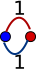
\includegraphics[width=0.05\linewidth]{binary_det.svg}}\label{fig:binary_det}
  \end{myenuma}
 \end{center}
  \caption{Synaptic models that maximize initial SNR.
  (\ref{fig:max_init_pot}) For potentiation, all transitions starting from a weak state lead to a strong state, and the probabilities for all transitions leaving a given weak state sum to 1.
  (\ref{fig:max_init_pot}) Depression is similar to potentiation, but with strong and weak interchanged.
  (\ref{fig:binary_det}) The equivalent two state model, with transition probabilities under potentiation and depression equal to one.
  }\label{fig:max_init}
\end{figure}


\subsection{Area}\label{sec:area}

Now consider the area under the memory curve:
%
\begin{equation}\label{eq:area}
  A = \int_0^\infty\!\!\dr t \, \snr(t).
\end{equation}
%
We will find an upper bound on this quantity as well as the model that saturates it.
The area is useful as it also provides an upper bound on the lifetime of a memory, $\tau(\epsilon)$, defined as the time at which $\snr(\tau)=\epsilon$ (we often take $\epsilon=1$):
%
\begin{equation}\label{eq:arealife}
  A = \int_0^\infty\!\!\dr t \, \snr(t)
    > \int_0^{\tau(\epsilon)}\!\!\dr t \, \snr(t)
    > \int_0^{\tau(\epsilon)}\!\!\dr t \, \epsilon
    = \epsilon \tau(\epsilon).
\end{equation}
%
However, the area still receives a contribution from the tail of the memory curve, after the SNR has decayed below any useful value.
This means that maximizing SNR will favor models with long tails that will not necessarily be good for storing memories.

One important property of the area is that it has a null ``scaling'' degree of freedom.
If all off-diagonal elements of $\M\potdep$ are multiplied by a constant, with diagonal elements adjusted to keep row-sums fixed, this will have two effects.
First, it will scale up the initial signal creation.
Second, it will scale down time.
Combining these two effects, it will leave the area invariant.

This feature allows us to ignore the lower bound on the diagonal elements, $\M\potdep_{ii}>0$.
If we maximize the area ignoring this constraint, the ``scaling'' mode can be used to satisfy it without changing the area.

We also develop an important organizing principle using the theory of first passage times.
The mean first passage time matrix, $\fptb_{ij}$, is defined as the average time it takes to reach state $j$ for the first time, starting from state $j$.
The diagonal elements are defined to be zero.
Then the quantity
%
\begin{equation}\label{eq:kemenyconst}
  \eta \equiv \sum_j \fptb_{ij}\eq_j
\end{equation}
%
is independent of the starting state $i$.
It is known as Kemeny's constant (see \cite[\S4.4]{kemeny1960finite}).
We can define analogous quantities
%
\begin{equation}\label{eq:kemenypm}
   \eta^+_i = \sum_{j\in+} \fptb_{ij} \eq_j,
   \qquad
   \eta^-_i = \sum_{j\in-} \fptb_{ij} \eq_j.
\end{equation}
%
These can be thought of as the average time it takes to reach the strong/weak states respectively.
We can put the states in order of decreasing $\eta^+_i$ or increasing $\eta^-_i$.
Because $\eta^+_i+\eta^-_i=\eta$ is independent of $i$, the two orderings are the same.

With the states in this order, we can find perturbations of $\M\potdep$ that will always increase the area, whilst leaving the equilibrium distribution, $\eq$, unchanged.
Some of these perturbations are shown in \autoref{fig:perts}.
The only thing that can prevent these perturbations from increasing the area is when they require the decrease of a matrix element that has already been set to 0.
This determines the topology (non-zero transition probabilities) of the model with maximal area.
It is of the form shown in \autoref{fig:max_area}, with potentiation moving one step to the right and depression moving one step to the left.
Any other topology would allow some perturbation to further increase the area.


\begin{figure}[tbp]
 \begin{center}
 \begin{myenuma}
  \item\aligntop{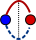
\includegraphics[width=0.1\linewidth]{triangular_right.svg}}\label{fig:tri_right}\hp
  \item\aligntop{\includegraphics[width=0.1\linewidth]{triangular_left.svg}}\label{fig:tri_left}\hp
  \item\aligntop{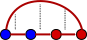
\includegraphics[width=0.2\linewidth]{shortcut.svg}}\label{fig:shortcut}
 \end{myenuma}
 \end{center}
  \caption{Perturbations that increase the area.
  (\ref{fig:tri_right}) Perturbations that increase elements of $\M\pot$ above the diagonal and decrease the corresponding elements of $\M\dep$. It can no longer be used when $\M\dep$ is lower triangular.
  (\ref{fig:tri_left}) Perturbations that decrease elements of $\M\pot$ below the diagonal and increase the corresponding elements of $\M\dep$. It can no longer be used when $\M\pot$ is upper triangular.
  (\ref{fig:shortcut}) Perturbation that decreases ``shortcut'' transitions and increases the bypassed ``direct'' transitions. It can no longer be used when there are only nearest-neighbor ``direct'' transitions.
  }\label{fig:perts}
\end{figure}

As these perturbations do not change the equilibrium distribution, this means that the area of \emph{any} model is bounded by that of a linear chain with the same equilibrium distribution.
This area is given by
%
\begin{equation}\label{eq:multistatearea}
  A \leq \frac{2\sqrt{N}}{r} \sum_k \brk{k - \sum_j j\eq_j} \eq_k \w_k
    = \frac{2\sqrt{N}}{r} \sum_k \abs{k - \sum_j j\eq_j} \eq_k ,
\end{equation}
%
where we chose $\w_k=\sgn\brk{k - \sum_j j\eq_j}$.
We can then maximize this by pushing all of the equilibrium distribution symmetrically to the two end states.
This can be done by reducing the transition probabilities out of these states, as in \autoref{fig:max_area}.
This makes it very difficult to get out of the end states once they have been entered.
The resulting area is
%
\begin{equation}\label{eq:max_area}
  A \leq \frac{\sqrt{N}(M-1)}{r}.
\end{equation}
%
This result is similar to that found numerically by Barrett and van Rossum \cite{Barrett2008discrete} in a slightly different situation.

The ``sticky'' end states result in very slow decay, but they also make it difficult to encode the memory in the first place.
The memory curve for this model starts off very low, but hovers above zero for a very long time.
This is also not a good design for a synapse, but the resulting bound on the area will also prove useful in \autoref{sec:env}.


\begin{figure}[tbp]
 \begin{center}
  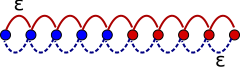
\includegraphics[width=0.4\linewidth]{multistate_sticky.svg}
 \end{center}
  \caption{Model that maximizes the area.
  Unlabeled transitions have probability 1.
  Labeled transitions have probability $\varepsilon\to0$.
  }\label{fig:max_area}
\end{figure}



\section{Memory curve envelope}\label{sec:env}

Now we will look at the implications of the upper bounds found in the previous section for the SNR at finite times.
As argued in \eqref{eq:SNReigen}, the memory curve can be written in the form
%
\begin{equation}\label{eq:SNRmodes}
  \snr(t) = \sqrt{N}\sum_a \CI_a \e^{-rt/\tau_a}.
\end{equation}
%
The upper bounds on the initial SNR, \eqref{eq:max_init}, and the area, \eqref{eq:max_area}, imply the following constraints on the parameters $\brc{\CI_a,\tau_a}$:
%
\begin{equation}\label{eq:modeconstr}
  \sum_a \CI_a \leq 1,
  \qquad\qquad
  \sum_a \CI_a \tau_a \leq M-1.
\end{equation}
%
We are not claiming that these are a complete set of constraints: not every set $\brc{\CI_a,\tau_a}$ that satisfies these inequalities will actually be achievable by a synaptic model.
However, any set that violates either inequality will definitely not be achievable.

Now we can pick some fixed time, $t_0$, and maximize the SNR at that time \wrt the parameters $\brc{\CI_a,\tau_a}$, subject to the constraints above.
This always results in a single nonzero $\CI_a$:
%
\begin{equation}\label{eq:env}
\begin{aligned}
  t_0 &\leq \frac{M-1}{r} &
   \implies 
  \snr(t) &= \sqrt{N}\e^{-rt/(M-1)} &
   \implies 
  \snr(t_0) &= \sqrt{N}\e^{-rt_0/(M-1)},\\
  t_0 &\geq \frac{M-1}{r} &
   \implies 
  \snr(t) &= \frac{\sqrt{N}(M-1)\e^{-t/t_0}}{rt_0} &
   \implies 
  \snr(t_0) &= \frac{\sqrt{N}(M-1)}{\e rt_0}.
\end{aligned}
\end{equation}
%
Both the initial SNR bound and the area bound are saturated at early times.
At late times, only the area bound is saturated.
The function $\snr(t_0)$, the green curve in \autoref{fig:env}(\ref{fig:envplot}), above forms a memory curve envelope.
No synaptic model can have an SNR that is greater than this at any time.
We can use this to find an upper bound on the memory lifetime, $\tau(\epsilon)$, by finding the point at which the envelope crosses $\epsilon$:
%
\begin{equation}\label{eq:lifebound}
  \tau(\epsilon) \leq \frac{\sqrt{N}(M-1)}{\epsilon\e r},
\end{equation}
%
where we assume $N>(\epsilon\e)^2$.

This leaves the question of whether this bound is achievable.
At any time, can we find a model whose memory curve touched the envelope?
The red curves in \autoref{fig:env}(\ref{fig:envplot}) show the closest we have come to the envelope with actual models, by repeated numerical optimization with random initialization and by hand designed models.

We see that here is a gap between the upper bound that we can prove and what we can achieve with actual models.
There may be other models we haven't found that could beat the ones we have, but it is probably too much to expect them to reach this envelope.
That would require saturating the area bound, and we saw that the only model that does that has very low initial SNR.
It seems that we need to find additional constraints to add to those we have \eqref{eq:modeconstr}, thereby bringing the envelope down.
We do not necessarily need to find \emph{every} constraint.
We have already seen that not every constraints is saturated for certain time ranges, so it may be that a small subset of them will be sufficient to find an envelope that is tight.






\begin{figure}
 \begin{center}
 \begin{myenuma}
  \item\aligntop{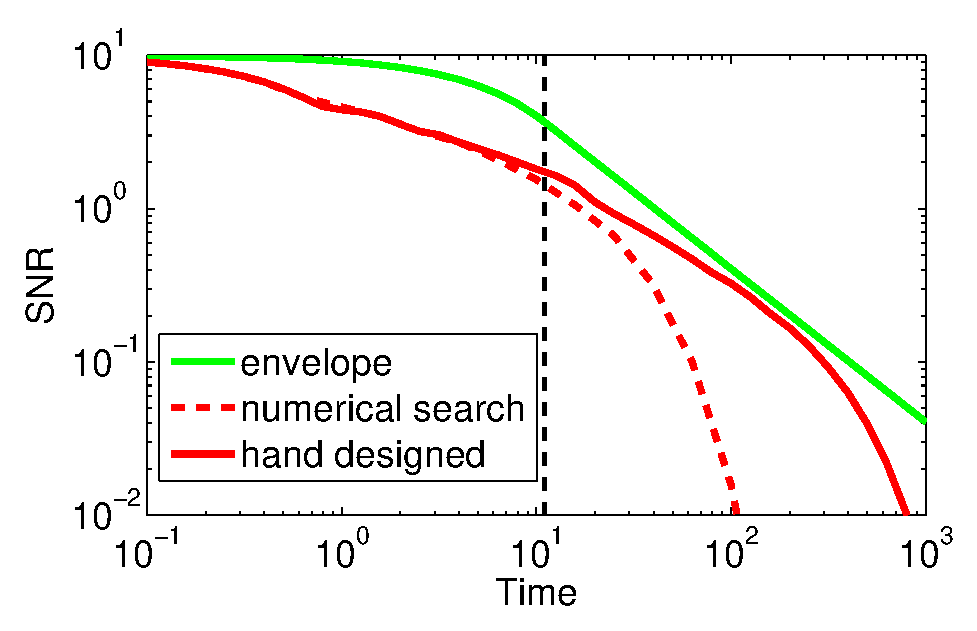
\includegraphics[width=0.4\linewidth]{env.eps}}\label{fig:envplot}\hp
  \item\aligntop{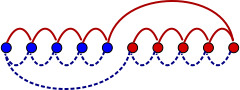
\includegraphics[width=0.3\linewidth]{diffjump.svg}}\label{fig:diffjump}
 \end{myenuma}
 \end{center}
  \caption{The memory curve envelope for $N=100$, $M=12$.
  (\ref{fig:envplot}) An upper bound on the SNR at any time is shown in green.
  The red dashed curve shows the result of numerical optimization of synaptic models with random initialization.
  The solid red curve shows the highest SNR we have found with hand designed models.
  At early times these models are of the form shown in (\ref{fig:diffjump}) with different numbers of states.
  At late times they are of the form shown in \autoref{fig:max_area} with different values of $\varepsilon$.
  }\label{fig:env}
\end{figure}







\section{Discussion}\label{sec:disc}





%\subsubsection*{Acknowledgements}


%%%%%%%%%%%%%%%%%%%%%%%%%%%%%%%%%%%%%%%%%%%%%%%%%%%%%%%%%%%%%%%%%%%%%%%%%%

\bibliographystyle{utcaps_sl}
\bibliography{maths,neuro}


\end{document}
